\chapter{背景}
\label{chap:relevantstudy}

本章では不完全情報ゲームの関連研究を述べ、麻雀の関連研究がどのように行われているかを述べる。


% \section{ゲーム木探索の背景}
% 探索の方法として一般的なのは、「mini-max探索」と呼ばれているもので、自らの手はできるだけ高い評価に、そこから想定される相手の候補手はできるだけ低い評価になるように探索していく。その結果を理想的な順番に並べ、可能性の低い選択肢を切り捨てる「αβ枝刈り」を行うことで、探索を効率化させることもできる。

% ただし不完全情報ゲームにおいてはこの方法では探索空間が広がりすぎて精度を保つことが出来ないので、別の解決策を考える必要があった。

% \begin{figure}[h]
%  \centering
%  \includegraphics[keepaspectratio, scale=1.0,bb=0 0 286 215]
%       {img/minimax.png}
%  \caption{mini-max探索}
%  \label{monte2}
% \end{figure}


\section{不完全多人数情報ゲームの例}
プレイ人数に着目した研究としてはポーカーを用いたもの \cite{poker},\cite{hurui} がある。これらの手法では 2 プレイヤでのゲームを強くしてから多人数に適応する方法がとられている。ポーカーは2 プレイヤであればナッシュ均衡戦略を用いることで世界チャンピオンに勝っているが、ポーカーは 2人から 10 人程度で参加可能なゲームであり人数が増える
と状態数が指数関数的に増大するためナッシュ均衡戦略の計算は難しい。そこで 2 人で行われたナッシュ均衡戦略を3 人限定で拡張する方法、プレイヤの行動を削減、抽象化することでより少ない人数の少ないゲームを想定する方法がとられた。

\section{麻雀の例}

麻雀においてのAI研究については機械学習を用いた水木ら\cite{miki}や北川ら\cite{kitakawa}の研究が報告されているが、いずれも平均プレイヤの実力に至っていない。一方、水上ら\cite{bakuuti}は1人麻雀プレイ ヤの学習に牌譜との一致を目指した平均化パーセプトロンを用い、平均プレイヤ以上の実績を収めている。

水上らの研究より、麻雀においてもプレイヤの人数を削減してから多人数に適用する方法は有効である可能性が高く、以後ゲームを単純化した1人麻雀に対しての研究が報告されている。
% 水上ら\cite{bakuuti}1人麻雀プレイ ヤの学習に牌譜との一致を目指した平均化パーセプトロンを用いた。麻雀の特徴量は非常に膨大なため、この方法が採用された。学習に使った教師信号は、麻 雀サイト天鳳 \cite{tenhou} において鳳凰卓でプレイすることができ るプレイヤの試合データである。鳳凰卓でプレ イできるのは全プレイヤの中でも上位 0.1%程度であり牌
% 譜の質は高いと考えられる。この研究では、1人麻雀プレイヤの和了率が平均プレイヤを上回り、鳳凰卓でプレイできるプレイヤの和了率に近いレベルになった。
% しかし、1人麻雀プレイヤの学習を行う際に、4人麻雀の牌譜を使っていることで、4人麻雀独特の打ち方を排除できない問題や、上級者が認知できない最適解を求められない問題があった。


% \section{人間プレイヤーの牌譜から学習する手法を用いた研究}
% 人間プレイヤーの牌譜を教師信号とした麻雀評価関数の機械学習の報告がいくつかなされている。
% 北川らは評価関数に 3 層ニューラルネットワークを用い た教師あり学習を用いることで麻雀 AI のパラメータ調整 を行った。\cite{kitakawa}牌譜と AI の一致率はツモ局面において約56%, 鳴き局面において約89%,東風荘で得られたレートは 1318 であった[6].
% 三木らは木カーネルを用いた非線形 SVM によって手牌 の分類を学習した.ツモ局面における人間プレイヤーとの 一致率は 51%であった\cite{miki}。
% しかし、いずれの方法も人間の平均プレイヤの実力に達していない。

% 水上ら\cite{bakuuti}1人麻雀プレイ ヤの学習に牌譜との一致を目指した平均化パーセプトロンを用いた。麻雀の特徴量は非常に膨大なため、この方法が採用された。学習に使った教師信号は、麻 雀サイト天鳳 \cite{tenhou} において鳳凰卓でプレイすることができ るプレイヤの試合データである。鳳凰卓でプレ イできるのは全プレイヤの中でも上位 0.1%程度であり牌
% 譜の質は高いと考えられる。この研究では、1人麻雀プレイヤの和了率が平均プレイヤを上回り、鳳凰卓でプレイできるプレイヤの和了率に近いレベルになった。
% しかし、1人麻雀プレイヤの学習を行う際に、4人麻雀の牌譜を使っていることで、4人麻雀独特の打ち方を排除できない問題や、上級者が認知できない最適解を求められない問題があった。



\section{麻雀についてモンテカルロ法を応用した研究}
\subsection{モンテカルロ法}

水上ら\cite{bakuuti}の研究の前衛である、「麻雀を打つ機械」\cite{nmizu}の牌効率のアルゴリズムでは、モンテカルロ木探索を用いている。
そのアルゴリズムの概要を図\ref{fig:monte2}に示す。
ツモを入れた状態で14枚の牌姿から、それぞれ切ることのできる牌を切った場合を一つのノードとする。この場合深さ1の14つのノードができることになる。
この後、それぞれのノードの状態から、ツモることの可能な牌をランダムにツモっていくシミュレーションを行う。この場合ツモる事のできる牌とは、場や自分の手牌に情報として見えている牌をゲーム開始時に存在する麻雀牌セットの中から抜いたものである。通常麻雀のルールでは、牌をツモることで次に捨てるという動作が発生するが、ここではそれを行わない。これをしないことで、探索空間が膨大に膨れ上がるの防ぐ効果があり、特定のシミュレーション時に最速で上がるための手順を特定することが可能となる。ツモを連続で行っていき、それまで手牌に残っていた牌の組み合わせで和了することができる場合となるまでシミュレーションを行い、上がった場合にプレイアウトとなる。このシミュレーションを各ノードでそれぞれ十分な回数行い、プレイアウト発生するまでのツモった回数の平均とり評価値とする。最後に、各ノードの評価値を比較し、最もこの値が少なかったノードが最適な打牌と考え選択することになる。プレイアウトまでにツモった回数の平均が少なければ少ないほど、より早く和了できることが期待されるからである。

\begin{figure}[h]
 \centering
 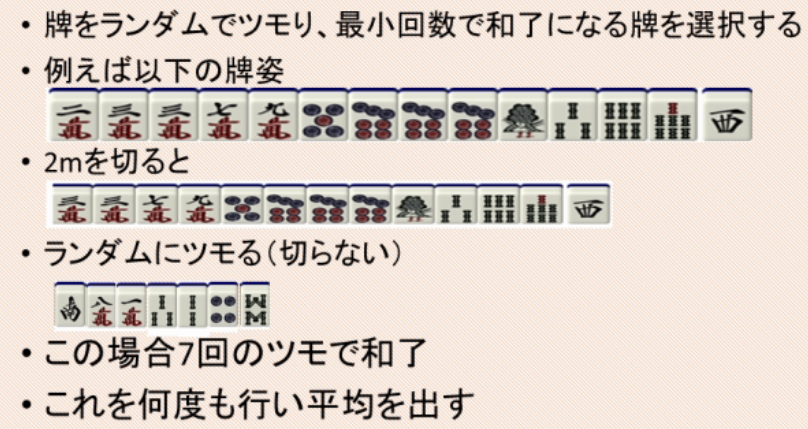
\includegraphics[keepaspectratio, scale=0.25,bb=0 0 808 429]
      {img/monte1.png}
 \caption{麻雀を打つ機械の牌効率アルゴリズム}
 \label{monte1}
\end{figure}

\begin{figure}[h]
 \centering
 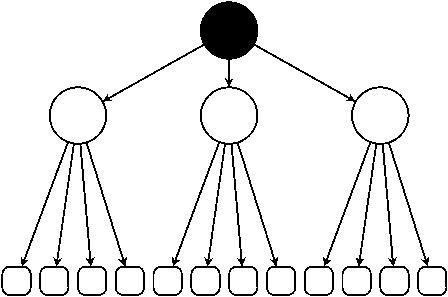
\includegraphics[keepaspectratio, scale=0.5,bb=0 0 283 121]
      {img/monte.jpg}
 \caption{モンテカルロ木探索}
 \label{monte2}
\end{figure}

\subsection{UCB1}
以上で述べたモンテカルロ法の問題点は、各ノードに対して行うシミュレーションがそれぞれ膨大なため、プレイアウトまでの回数が多く精度が落ちてしまうことである。
この問題を解決するために、提案されている手法の中に、Upper Confidence Bound (UCB) \cite{UCB}を用いたものがある。
UCB ではある局面から考えられる全ての手に対して, よい結果 を返しそうな手を重視しつつ、何度もプレイアウトと呼ば れるランダムシミュレーションを行うことで 最善の手を決定する手法である。有望な手に対して多くのプレイアウトを実行することで、先に述べた通常のモンテカルロ木探索よりも精度を上げることができる。以下、このアルゴリズムを詳しく説明する。

通常のモンテカルロ木探索では、ノードごとに期待される手の良さを途中で判定していないため、全てのノードに対して同じ回数のプレイアウトを行うことになる。したがって、良い手が期待できないノードに対しても多くのプレイアウトを割り当てることになり、無駄なシミュレーションを行ってしまう事が考えられる。また、ノードによっては手の良さを決定する分岐がプレイアウトに対して大量にある場合、他のノードと同じ回数のプレイアウトでは十分な評価が出来ない可能性もある。このような問題に対して、UCBでは、UCB1値を用いることによって各ノードの有望さをその都度確認し、全体のプレイアウトの回数や特定のノードで行われたプレイアウトの回数を考慮して、プレイアウトをどのノードに数多く割り当てるかということを判別することを考える。
UCB1値は、${x_{j}}$は子ノード$j$の平均報酬, $α$は定数,$n$は親ノードの探索回数, ${n_{j}}$は子ノード$j$とした時、

\begin{equation}
\label{UCB1value}
\Large UCB1 = \overline {x_{j}}+\alpha \sqrt {\displaystyle \frac {2\log{n}} {n_{j}}}
\end{equation}
で表される。
式 \ref{UCB1value}の右辺の第 1 項は平均報酬を, 第 2 項は信頼度を示している。従来のモンテカルロ木探索では第1項の平均報酬をそのまま全てのプレイアウトが終了するまで行った値として利用していたが、UCB1ではここで第2項の信頼度を用いることで全てのプレイアウトが終了するよりも前に信頼できる範囲を推定する。そうすることで、多くのプレイアウトを最後まで割り当てなくとも、一定の信頼度で少ないプレイアウトでそのノードが有望かどうかを判別することが可能になる。
信頼度はそのノードのプレイアウト回数が少ないと大きく, 多いと小さくなる。UCB1 値を用いることでUCB1 ではよ り有望そうな手に対して多くのシミュレーションを行う事 ができる。

\begin{figure}[h]
 \centering
 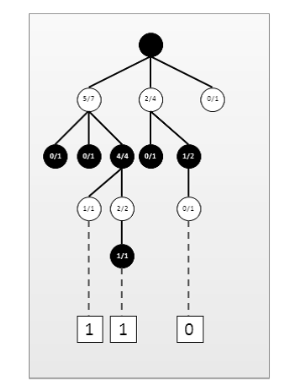
\includegraphics[keepaspectratio, scale=0.75,bb=0 0 304 387]
      {img/UCB.png}
 \caption{UCBを用いたモンテカルロ木探索}
 \label{monte2}
\end{figure}

\subsection{Lin UCB}
UCB1 は各局面ごとにこの手順を実行するが, 各局面を完全に異なる局面として扱うため, 他の局面の探 索において得られた情報を共有することができないという 欠点を持つ. この欠点を補うアルゴリズムとして期待され ているのが LinUCB である.

UCB は局面ごとにこの探索を実行するが, 各局面を完全 に別の局面として扱うため他の局面の探索において得た情 報を利用することができない。この問題を解決するためにLinear UCB (LinUCB) \cite{LinUCB} という手法が提案されている。これは、局面を特徴で表す ことで、対象とする局面が異なっても, それまで対象とした局面の情報を利用できるといったものである。

LinUCB [5] は, UCB を局面を特徴で表すことができる ように拡張したものであり, 牌譜の局面からの教師あり学 習や異なる探索の結果の共有ができる手法である。
LinUCB はプレイアウトを行う子ノードを選択する評価値の計算に, 重みベクトル, 特徴ベクトル, 特徴の頻度を表す相関行列を 用いる. 計算により求めた評価値が最大となる子ノードに 対してプレイアウトを行い, 共通で保持する重みベクトル を更新する. 重みベクトルは, 選択したノードの特徴ベクト ルの各項にプレイアウト結果の報酬を乗じた値を, 重みベ クトルの対応する項に足し込んで更新する. この更新によ り, 高い報酬を得た特徴は大きな重みを, 低い報酬の特徴は 小さな重みを持つようになるため, 当該ノードだけでなく, 同様の特徴を持つ他のノードの評価値も更新される. これ により異なる局面で得られた情報を共有し, 利用すること ができる. また LinUCB は探索を行った結果を重みベクト ルとして記録しておくことで, 事前学習の結果を用いる探 索として利用することも可能である.
LinUCB のアルゴリズムを Algorithm 1 に示す. ただし xt,at はプレイアウト回数が t 回目の時の選択肢 a の特徴ベ クトル, A は特徴の共起を含めた頻度を表す相関行列, b は
各ノードごとの報酬の総和を表すベクトル, θt は重みベク トル, pt,a は選択肢 a の評価値, α はバランスパラメータ, rt は報酬を表している. rt はプレイアウトにより与えるか, 学習データにより与えるものとする. LinUCB は 4 行目で 前回のプレイアウト結果を反映して重みベクトル θt を更 新する. 7 行目で重みベクトル, 特徴ベクトル, 相関行列を 用いて各ノードの評価値を計算し, 9 行目で評価値が最大 となるノードを選択する. 10 行目でプレイアウトを行い報 酬を受け取り, 11 行目, 12 行目で A と b の更新を行う.
LinUCB は Algorithm 1 の 7 行目に示したように, 式 (2) により各ノードの評価値を求める. 式 (2) の第 1 項は各ノー ドの平均報酬を計算しており, 第 2 項で信頼度を計算して いる.
\begin{equation}
\label{LinUCB}
\Large pt,a = θTt xt,a + α
\end{equation}
また, UCB で用いている評価値も, 平均報酬と信頼度の和 で計算される. つまり LinUCB と UCB は本質的に等しい 計算をしていることが分かる. また, LinUCB の第 2 項は データ数の増加により十分速く小さくなることが保証され ている [5]. 以上より, LinUCB は UCB と近い運用を行う ことができると考えられる.

これらは麻雀について適用した例が報告されている\cite{LinUCB_mahjong}が、いずれの方法も平均プレイヤーに満たない成績となった。

\section{本論文が着目する課題}
1人麻雀においてある局面からゲーム木を展開しようとした場合、次にどの種類牌をツモるかはわからないため、ランダムに決定しノードを展開していくことになる。これを繰り返し行うと探索空間が大きくなりすぎるため、手の選択が難しくなる。これを対処するために、あらゆる手法が提案されている。このような場合に木を展開せずに有望な手を選択する手法として、Upper Confidence Bound (UCB) \cite{UCB}がある。UCB ではある局面から考えられる全ての手に対して, よい結果 を返しそうな手を重視しつつ、何度もプレイアウトと呼ば れるランダムシミュレーションを行うことで 最善の手を決定する手法である。
UCB は局面ごとにこの探索を実行するが, 各局面を完全 に別の局面として扱うため他の局面の探索において得た情 報を利用することができない。この問題を解決するためにLinear UCB (LinUCB) \cite{LinUCB} という手法が提案されている。これは、局面を特徴で表す ことで、対象とする局面が異なっても, それまで対象とした局面の情報を利用できるといったものである。以上のような対策が考えられてはいるが、1人麻雀について適用した結果平均プレイヤーの実力までに至っていない。囲碁においては一定の成果を上げたものの、麻雀ではうまく適用できない問題に対しては、麻雀の場合はより探索の空間が大きく、UCB1値やLinUCBを指標とするノードの展開の方法ではうまく適用できていない可能性がある。したがって本研究では、ノードの展開を行う際に指標とするものを麻雀というゲームの性質上の状況のパラメーターを用意し、それを使うこととする。

% しかし、UCB1 と LinUCB の評価値計算において信頼度の 計算式が異なることや、特徴量の設計に問題があるなどの理由でいい結果は出ていなかった。 
